% !TEX root = ../eval.tex

\section{Alternative specifications}%
\label{sec:alternative_control_group_designs}

\subsection{Static TWFE}%
\label{sub:static_twfe}

\begin{equation}
    y_{it} = \alpha_i + \lambda_t + \beta T_{it} + \gamma X_{it} + \epsilon_{it}
\end{equation}

\begin{itemize}

    \item Comparison: pre vs post signup within each individual.

    \item Assumption: there are no time-varying unobserved effects that affect
        both y and T.

    \item Discussion: there is something that made the individual sign up in
        the first place, and it might well be an individual level shock that we
        don't observe (unexpected large expense, loss of job, etc.)

    \item See \citet{imai2021use} for problems with twfe
\end{itemize}


\subsection{Dynamic TWFE}%
\label{sub:dynamic_twfe}

\begin{equation}
    y_{it} = \alpha_i + \lambda_t + \sum^{5}_{s=-6} \beta_s T_{its} + \gamma X_{it} + \epsilon_{it}
\end{equation}

\begin{itemize}
    \item See \citet{sun2021estimating} for problems with that and compare to
        their approach as implemented in fixest.
\end{itemize}

\subsection{Alternative window lengths}%
\label{sub:alternative_window_lengths}

Show results for 12 months on either end.

\subsection{Alternative matching method}%
\label{sub:alternative_matching_method}

\subsection{Post treatment periods as control}%
\label{sub:post_treatment_periods_as_control}

\subsection{Synthetic controls}%
\label{sub:synthetic_controls}

See \citet{abadie2021penalized} for how to use synthetic controls for disaggregated data.

\subsection{Classic two-way fixed-effects model}%
\label{sub:classic_two_way_fixed_effects_model}


\begin{figure}[htpb]
    \centering
    \caption{Naive pre-post results}%
    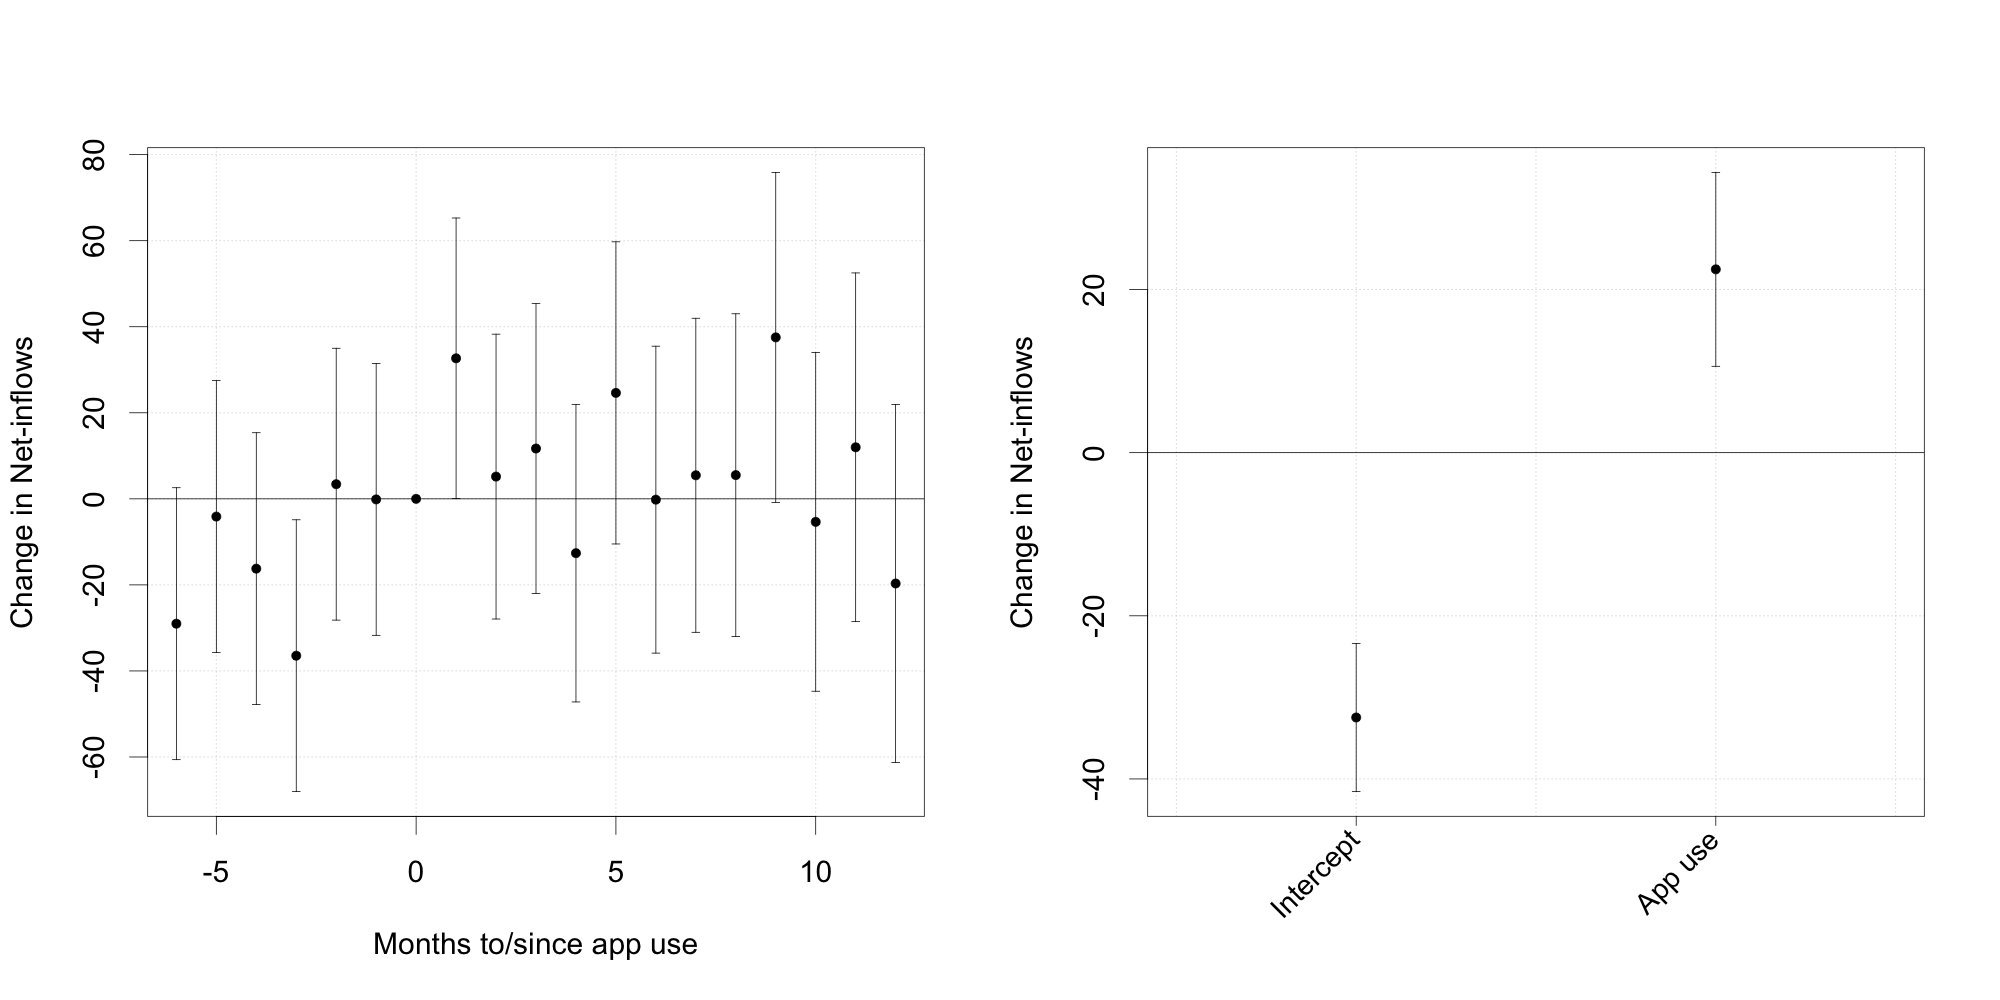
\includegraphics[width=\linewidth]{\figdir/reg_naive_pre_post.png}
    \label{fig:reg_naive_pre_post}
    \fignote{\textwidth}{Notes: ...}
\end{figure}

\begin{figure}[htpb]
    \centering
    \caption{Pre-post with controls}%
    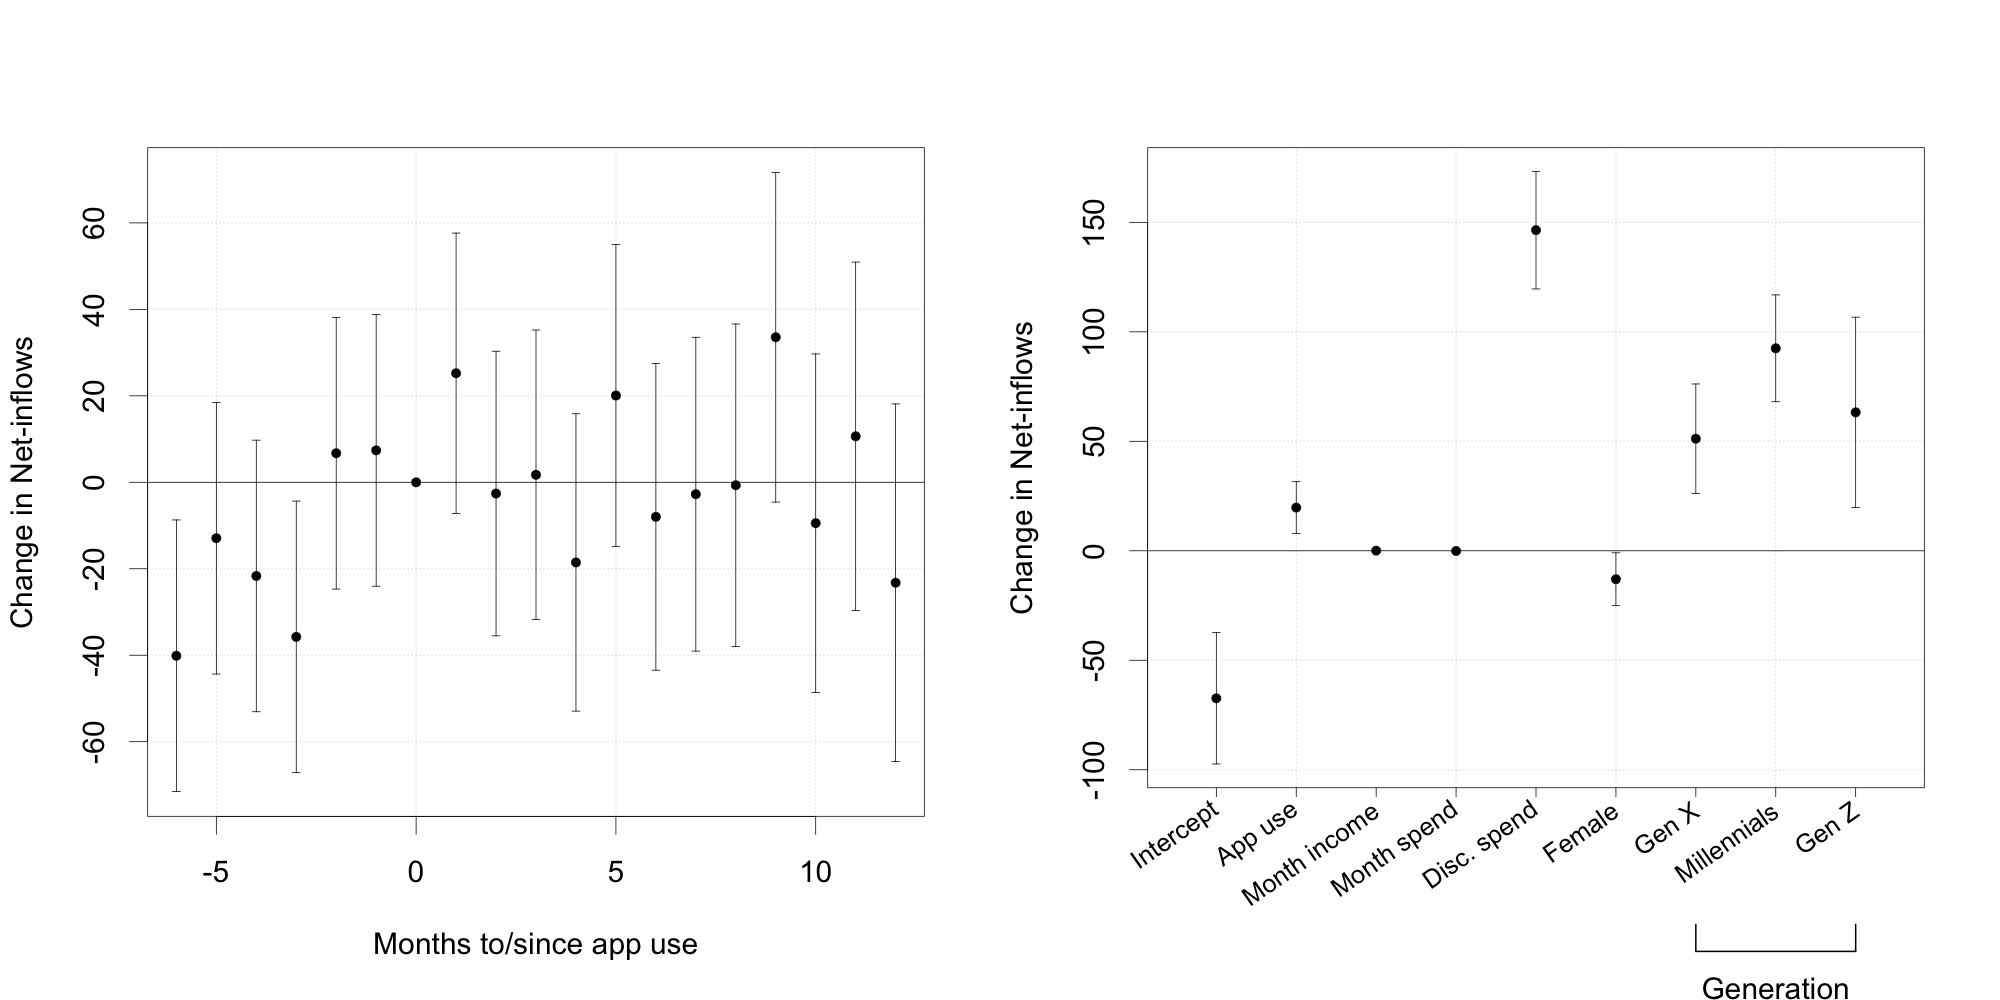
\includegraphics[width=\linewidth]{\figdir/reg_controls.png}
    \label{fig:reg_controls}
    \fignote{\textwidth}{Notes: ...}
\end{figure}

\begin{figure}[htpb]
    \centering
    \caption{TWFE}%
    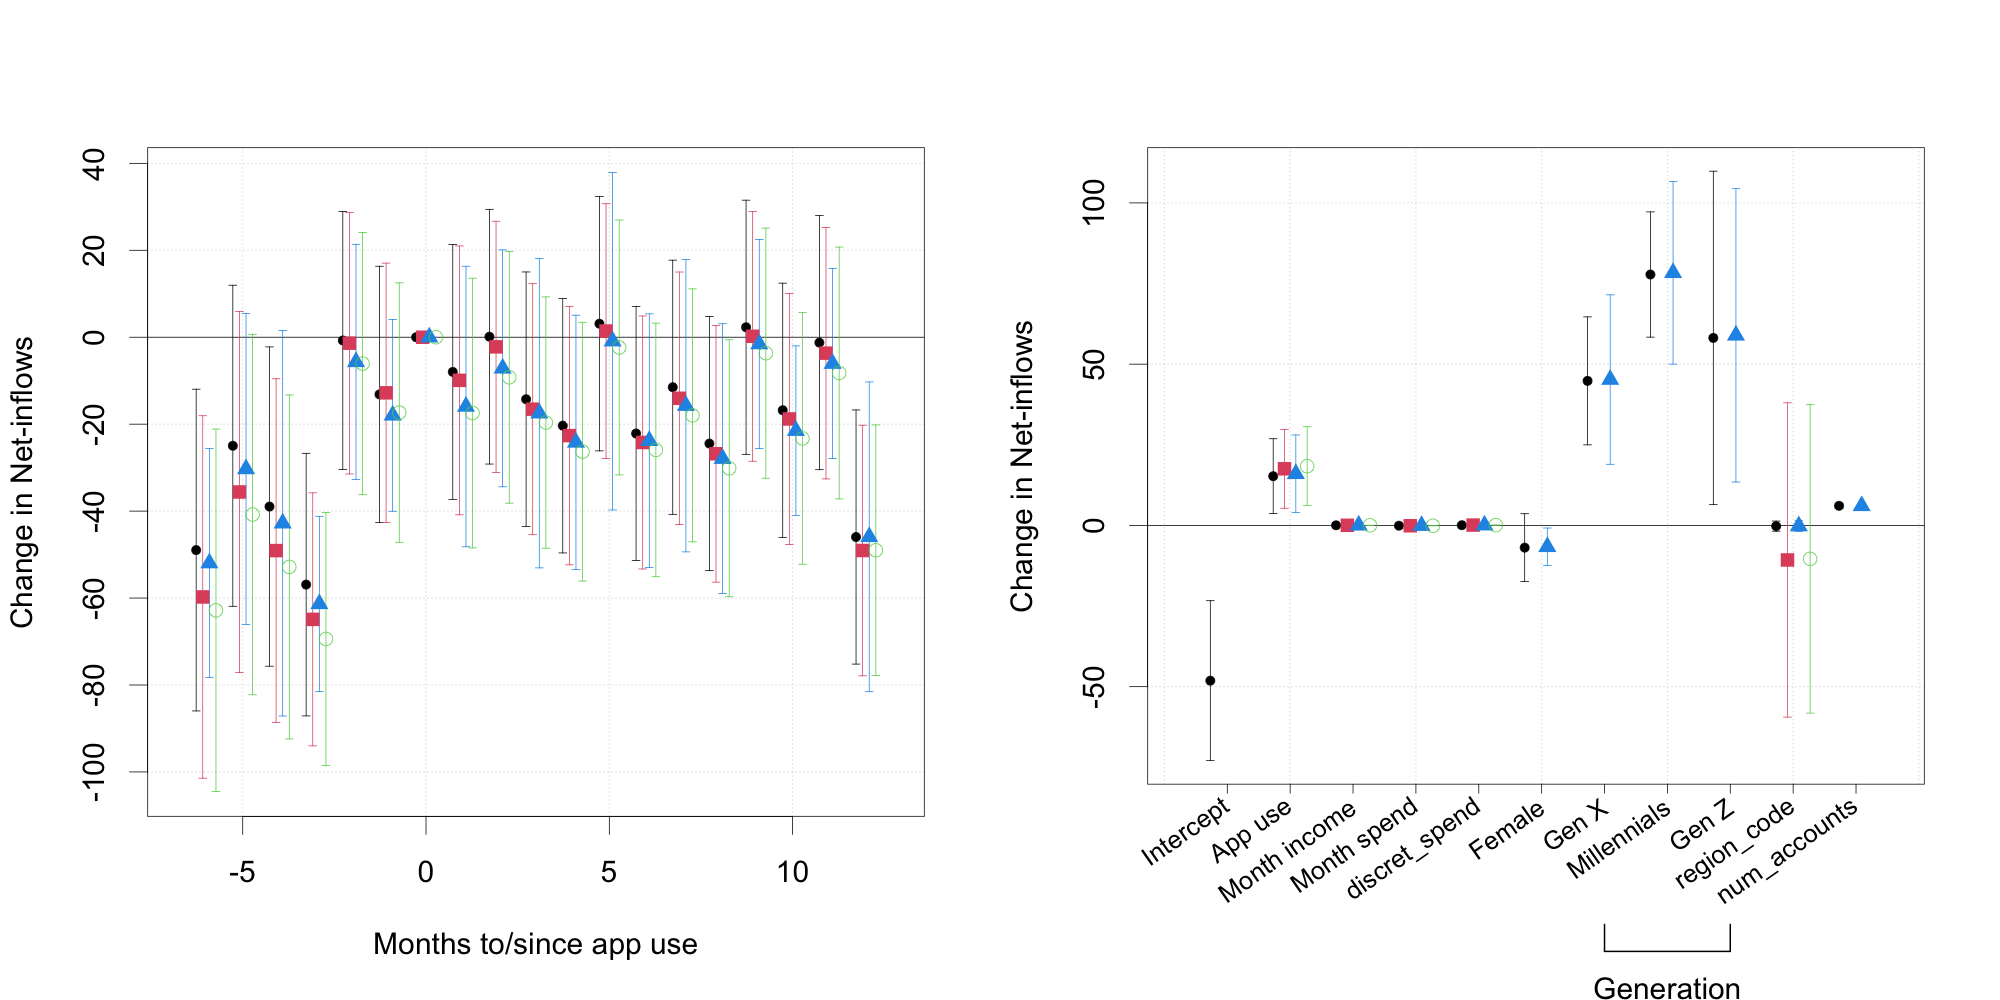
\includegraphics[width=\linewidth]{\figdir/reg_twfe.png}
    \label{fig:reg_twfe}
    \fignote{\textwidth}{Notes: ...}
\end{figure}

\begin{figure}[htpb]
    \centering
    \caption{Comparison}%
    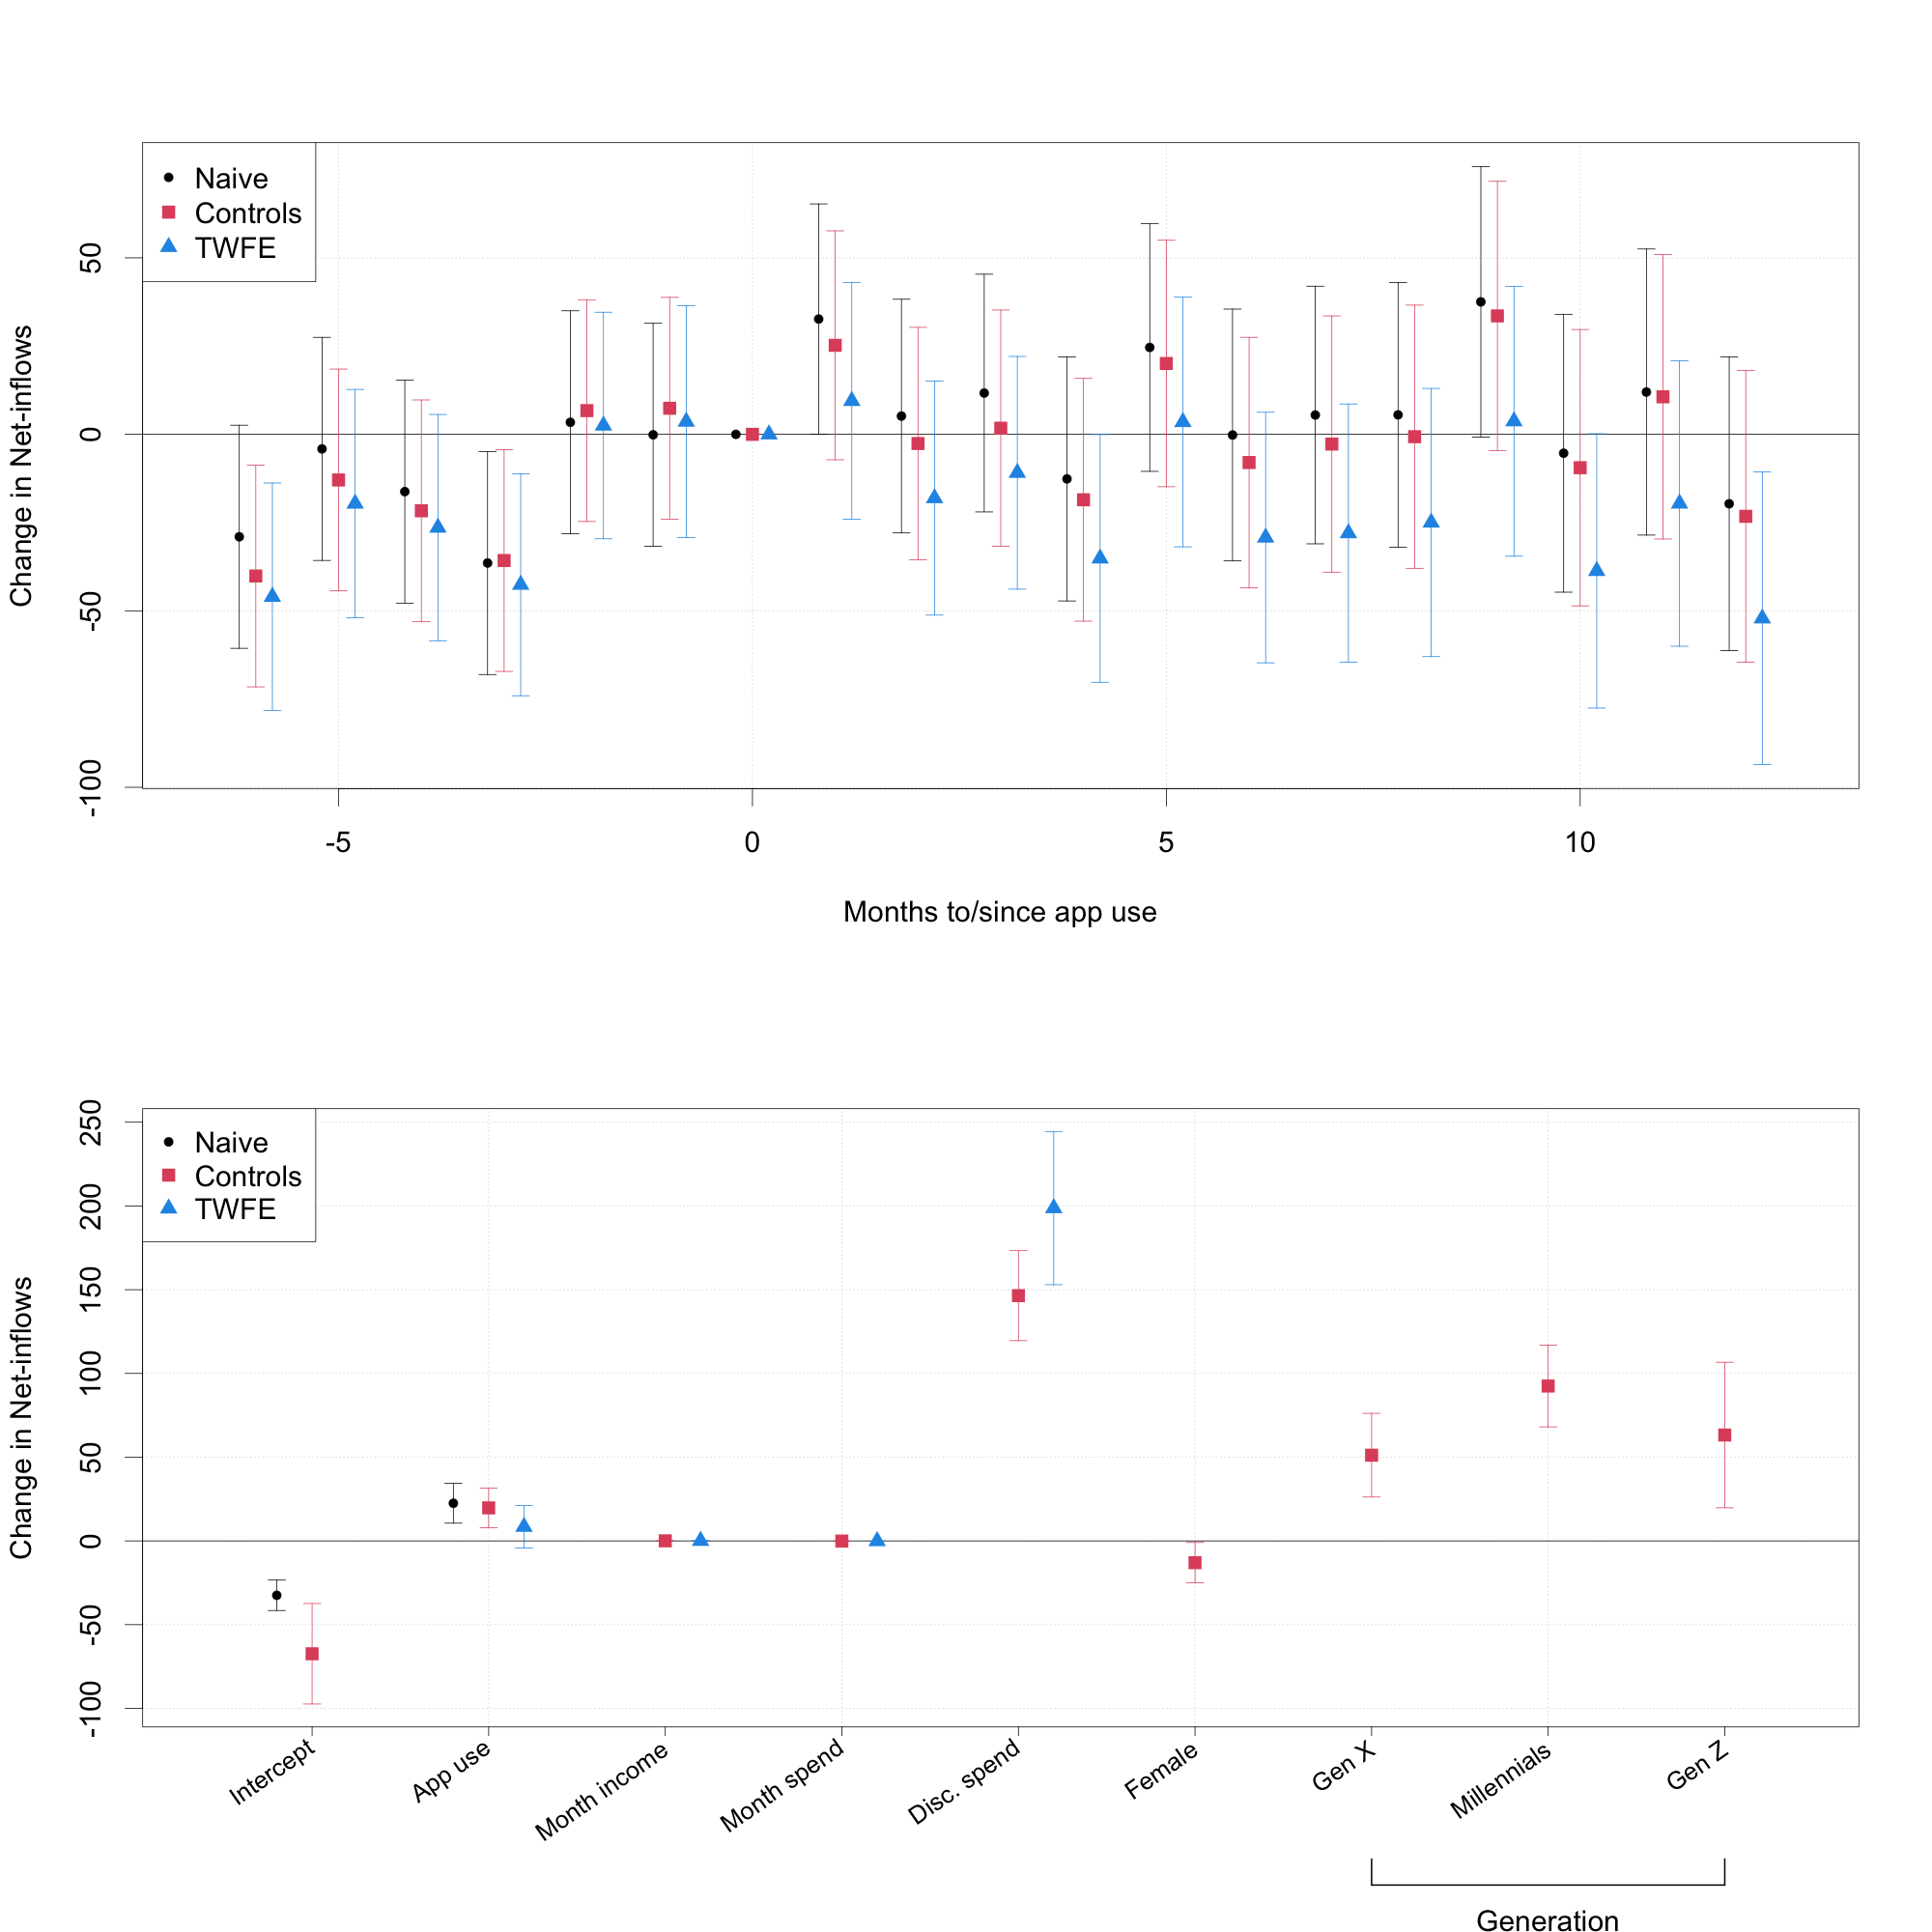
\includegraphics[width=\linewidth]{\figdir/reg_comparison.png}
    \label{fig:reg_comparison}
    \fignote{\textwidth}{Notes: ...}
\end{figure}
